% !TeX root = ADP-SG.tex

\chapter{Problem and Approaches to Solution}\label{ch:ProblemsMethods}

This chapter introduces the classical revenue management problem of capacity control problem under customer choice behaviour as can be found e.g. in \cite{Koch.2017} or in \cite{Strauss.2018}. It consists of deciding which products to offer at a given point in time and \Cref{s:Prob} gives a general description of the problem as well as a formulation as a dynamic program. Various methods of solving the problem are laid out in \Cref{s:Metho}.

\section{The problem}\label{s:Prob}

In this section, we describe the capacity control in general in \Cref{ss:Prob:GenDesc}, present a concrete example in the airline setting in \Cref{ss:Prob:AirDesc} and introduce the formulation of the resulting choice based capacity control model as a dynamic program in \Cref{ss:Prob:FormDynProg}. \todo{Subsection zu Problemen in der Lösung einfügen, die überleitet zu den verschiedenen Lösungsmethoden}

\subsection{General description}\label{ss:Prob:GenDesc}

A company offers a bundle of products to heterogeneous customers arriving over time. Products often correspond to services that have to be delivered at a given point in time. The period of time from now until delivery is referred to as selling horizon (or booking horizon), is considered finite and is split into a finite set of consecutive time points. The set of available products is also assumed to be finite and without loss of generality (w.l.o.g.\nomenclature{w.l.o.g.}{without loss of generality}) constant over time\footnote{If the set of available products change over time, let $S_t$ denote the set of available products at time $t$ and let $\mathcal{T}$ represent the finite set of time points. Then, $S \coloneq \cup_{t \in \mathcal{T}}S_t$ is again finite (finite union of finite sets) and can be taken as the constant set of available products at each time point.}. Each individual product is characterized by a given price and usage of a certain, finite, set of resources. These resources might be shared among different products. 

The goal of companies operating in the capitalistic society is to increase profits, which is equivalent to maximizing revenue in a specific setting. As stated, the price of individual products (leading to revenue) is assumed to be fixed, which is a realistic assumption for short terms considering potentially large costs coming with a change of price (e.g. selling products via catalogue). Furthermore, capacities are fixed in the short term (costly to increase production as e.g. more employees have to be hired) and are considered perishable. Often, capacity comes with high fixed costs and low marginal costs resulting from selling an additional product at any price (e.g. costs for operating one flight with 97 customers are mostly the same as for operating the same flight with 98 customers). Such a profit and cost structure justify the usage of revenue as a proxy for profit \cite{Strauss.2018}.

Switching to the customer side, the consideration of a heterogeneous customer group allows for modelling most real world scenarios. Not every customer is the same, but it is certainly reasonable to combine individuals to groups sharing similar characteristics. Some characteristics will be more prevalent in the overall population (more precise, the population that represents all persons interested in the companies' products).  Different customers have varying needs, thus different preferences and different willingness-to-pay leading ultimately to different purchases depending on the currently offered set of products. Thus, the company can influence the sales process by altering the offered set of products over the booking horizon, which is exactly the task of capacity control under customer choice behaviour.

\subsection{Description in airline setting}\label{ss:Prob:AirDesc}

An airline company operates a flight network connecting cities A, B and C as depicted in \Cref{fig:AirDesc}. The booking horizon consists of 20 time steps (e.g. today is Monday, booking is possible four times every day until and including Friday and flights depart on Saturday). The products to be offered are summarized in \Cref{tb:AirDesc:Prod}. Note that two products are available on Leg 1, i.e. the expensive product 1 and the less expensive product 2 (e.g. due to separate business and economy classes). A sell of either product 1 or product 2 will result in the reduction of available capacity on Leg 1 by one unit. Furthermore, product 6 presents an option to get from city A to city C (via city B) and thus a sell of product 6 results in a reduction of both Leg 1 and Leg 2 by one unit. Also product 4 is connecting city A and city C (on the direct flight) but is more expensive then product 6 (e.g. the company assumes the shorter travel time is of value to some travellers). 

Furthermore, capacities are presented in \Cref{tb:AirDesc:Res}, so there are eight available seats on Leg 1, but just four seats are available on Leg 2. Customers are characterized as stated in \Cref{tb:AirDesc:Cust}, so most customers belong to segment 1 (higher value of $\lambda_l$ representing larger size of customer segment $l$) and want to travel from city A to city B and prefer the budget option (as the value of preference for the latter product is much higher and a higher value corresponds to a higher preference). Customers belonging to segment 2 also want to travel from A to B, but are price insensitive, as they value the higher comfort of the more expensive product 1 just little higher as the cheaper product 2. Business customers that need to travel from A to C are represented by customer segment 3 as can be seen by the low preference for no purchase. 

\todo{Idee: Beschreibung der Customer Segmente könnte man zu \enquote{Persona} ausweiten}
\begin{figure}
	\caption{Working example for illustration of ideas with $T=20$ time periods.}
	\begin{subfigure}[t]{.3\linewidth}
		\centering
		\caption{Airline network. \label{fig:AirDesc}}
		\begin{tikzpicture}[
		mycircle/.style={
			circle,
			draw=black,
			fill=gray,
			fill opacity = 0.3,
			text opacity=1,
			inner sep=0pt,
			minimum size=20pt,
			font=\small},
		myarrow/.style={-Stealth},
		node distance=0.6cm and 1.2cm
		]
		\node[mycircle] (cB) {$B$};
		\node[mycircle,below left=of cB] (cA) {$A$};
		\node[mycircle,below right=of cB] (cC) {$C$};
		
		\foreach \i/\j/\txt/\p in {% start node/end node/text/position
			cA/cB/Leg 1/above,
			cB/cC/Leg 2/above}
		\draw [myarrow] (\i) -- node[sloped,font=\small,\p] {\txt} (\j);
		\draw[myarrow]([yshift= 20pt] cA) -- node[sloped,font=\small,above] {Leg 3} ([yshift= 20pt] cC);
		\draw[myarrow]([yshift= -20pt] cC) -- node[sloped,font=\small,below] {Leg 4} ([yshift= -20pt] cA);
		\end{tikzpicture}
	\end{subfigure}%
	\quad
	\begin{subtable}[t]{.4\linewidth}
		\caption{Products. \label{tb:AirDesc:Prod}}
		\small
		\centering
		\begin{tabular}{yxz}
			\toprule
			\text{Product} & \text{Origin-destination} & \text{Fare}\\
			\midrule
			1 & A \rightarrow B & 5\\
			2 & A \rightarrow B & 3\\
			3 & B \rightarrow C & 5\\
			4 & A \rightarrow C & 12\\
			5 & C \rightarrow A & 10\\
			6 & A \rightarrow B \rightarrow C & 8\\
			\bottomrule
		\end{tabular}
	\end{subtable}%
	\quad
	\begin{subtable}[t]{.2\linewidth}
		\caption{Resources. \label{tb:AirDesc:Res}}
		\small
		\centering
		\begin{tabular}{yy}
			\toprule
			\text{Leg} & \text{Capacity}\\
			\midrule
			1 & 8\\
			2 & 4\\
			3 & 4\\
			4 & 8\\
			\bottomrule
		\end{tabular}
	\end{subtable}
	
	\begin{subtable}{\linewidth}
		\caption{Customers.\label{tb:AirDesc:Cust}}
		\small
		\centering
		\begin{tabular}{lccccc}
			\toprule
			Seg. & $\lambda_l$ & \specialcell[b]{Consideration\\tuple\footnote{Note that in contrast to \cite{Bront.2009}, we use the mathematically correct terminology as \emph{tuple} does have an inherent order, while \emph{set} does not (and thus makes no mathematical sense to be combined with a preference vector referring to the order of products in the set).}} & \specialcell[b]{Preference \\vector} & \specialcell[b]{No purchase \\preference} & Description\\
			\midrule
			1 & $0.3$ & $(1, 2)$ & $(4, 8)$ & $2$ & Price sensitive, (A$\rightarrow$B)\\
			2 & $0.2$ & $(1, 2)$ & $(6, 5)$ & $2$ & Price insensitive, (A$\rightarrow$B)\\
			3 & $0.2$ & $(4, 6)$ & $(8, 4)$ & $1$ & Price sensitive, fast (A$\rightarrow$C)\\
			4 & $0.1$ & $(5)$ & $(2)$ & $2$ & Opportunity traveller, (C$\rightarrow$A)\\
			\bottomrule
		\end{tabular}
	\end{subtable}
\end{figure}


\subsection{Formulation as dynamic program}\label{ss:Prob:FormDynProg}

\subsubsection{Firm's perspective}

\begin{boxStefan}
	\begin{enumerate}
		\item time index always at the top
		\item index for products always at bottom
	\end{enumerate}

	Anständiges Symbolverzeichnis, z.B. mit glossaries \url{https://ctan.org/pkg/glossaries}
	
	Wertebereich der Variablen
\end{boxStefan}

\todo{Übersichtsliteratur \cite{Phillips.2011} anschauen (nur an Uni Augsburg, nicht an TUM)}

Extensive literature deals with revenue management and came up with formal notation suitable for the analysis of capacity control models. Good overviews can be found in \cite{Klein.2008} or in \cite{Phillips.2011}. In this thesis, we introduce notation for a capacity control model first under a general discrete choice model of demand and then directly using a multinomial logit model of demand. Notation is closely linked to \cite{Koch.2017} and the standard representation is used for a better orientation with the main ideas outlined in \Cref{tb:Prob:Notation}

\todo{Idee: Notation vereinheitlichen, stets ähnlich zu $t=1, \dots, T$. Also z.B. statt $j=1,\dots,n$ für Produkte auch $j=1,\dots,J$}
\todo{Notation: Change transpose to $\backslash$ text\{T\}}
\begin{table}
	\caption{Idea of notation}\label{tb:Prob:Notation}
	\begin{tabular}{cll}
		\toprule
		Symbol & Characteristic & Meaning\\
		\midrule
		$i, j, h, t, l, p$ & general small letter & index\\
		$n, m$ & specific small letters & maximum index\\
		$T, L$ & general capital letter & maximum index\\
		$S$ & {\color{red}specific capital letter} & tuple of elements\\
		$x_1$ & small with index & single number\\
		$\boldsymbol{x}$ & small and bold & vector\\
		$(x_1, \dots, x_n)$ & parenthesis around single numbers & row vector\\
		$(\dots)^T$ & $T$ on upper side & transpose\\
		
	\end{tabular}
\end{table}

First, we present the situation with its inflexible components. Consider a firm that produces $n$ distinguishable products indexed by $j = 1, \dots, n$. We already introduce the notation $[n] \coloneqq \{1, \dots, n\}$. Product $j$ comes with a certain price leading to a revenue of $r_j$ when the product is sold. The revenues are bundled by the vector $\boldsymbol{r} = (r_1, \dots, r_n)^T$. A total of $m$ different resources are used for production, which are indexed by  $h \in [m]$. In order to produce one unit of product $j$, certain resources are needed and the consumption of resources is captured by the vector $\boldsymbol{a}_j = (a_{1j}, \dots, a_{mj})^T$ are necessary, with $a_{hj}=1$ if resource $h$ is needed for production of product $j$ and $a_{hj} = 0$ otherwise. The resource consumption can be aggregated in the incidence matrix $A = (a_{hj})_{h\in [m], j \in [n]}\in {0, 1}^{m \times n}$. Additionally, the firm already identified the group of potential customers and segmented this group into a total of $L$ customer segments, which are indexed by $l \in [L]$. A customer of segment $l$ arrives with probability $\lambda_l$ and this parameter can be adjusted such that it matches the reality (e.g. there are two times as many customers belonging to segment $a$ then there are of segment $b$, so we choose $\lambda_a = 2\lambda_b$ ) and the model assumptions (only one customer arrives during each period).
\todo{Skalierung und Einflüsse auf Ankunftsraten in Fußnote oder Appendix}
\todo{Ergänzung: Beweis zu arrival probabilities können aufsummiert als kleiner gleich 1 angenommen werden, da der Parameter eines Poisson Prozesses dessen erwartete Ankunftszeit (? eig höher => mehr Leute kommen) beschreibt und damit mit der Feinheit der Zeitschritte angepasst werden kann. Poisson Prozess in \cite{Bront.2009} 3. Model
You just heard that the Poisson distribution is a limit of the Binomial distribution for rare events. This makes sense if you think about the stories. Say we do a Bernoulli trial every minute for an hour, each with a success probability of 0.1. We would do 60 trials, and the number of successes is Binomially distributed, and we would expect to get about 6 successes. This is just like the Poisson story we discussed in the video, where we get on average 6 hits on a website per hour. So, the Poisson distribution with arrival rate equal to np approximates a Binomial distribution for n Bernoulli trials with probability p of success (with n large and p small). Importantly, the Poisson distribution is often simpler to work with because it has only one parameter instead of two for the Binomial distribution.
The means are all about the same, which can be shown to be true by doing some pen-and-paper work. The standard deviation of the Binomial distribution gets closer and closer to that of the Poisson distribution as the probability p gets lower and lower. }. 

The finite time period from when booking is possible for the first time to when it is possible for the last time is discretized into a total of $T$ sufficiently small time periods, such that in each individual time period at most one customer arrives. Time periods are indexed by $t \in [T]$. To be very precise (particularly relevant for correct implementation), booking itself is just possible at beginning of each time period, i.e. for time period $t$, booking is possible at time point $t-1$. Furthermore, one customer purchases at most one product. 

Second, we look at the flexible components of the model, i.e. those components that might change over time. Initially, i.e. at the start of the first time period (time point 0), the available capacity of resource $h$ is given by $c_h^0$ and thus all available capacities are described by the vector $\boldsymbol{c}^0 = (c_1^0, \dots, c_m^0)^T$. 

Let us now explore what happens if product $j$ is purchased during time period $t$, i.e. at time point $t-1$. The old capacity vector is given by $\boldsymbol{c}^{t-1}$. As product $j$ claims capacities according to $\boldsymbol{a}_j$,  the capacity vector reduces accordingly to $\boldsymbol{c}^{t} = \boldsymbol{c}^{t-1} - \boldsymbol{a}_j$. Time moves forward, such that the last selling might occur at time period $T$, i.e. at time point $T-1$.

Time period $t$ can be seen as the following half open interval between time points: $(t-1, t]$.

\begin{figure}
	\caption{Visualization of the booking horizon with its time periods.\label{fig:Prob:Horizon}}
	\centering
	\begin{tikzpicture}[snake=zigzag, line before snake = 5mm, line after snake = 5mm]
	% draw horizontal line   
	\draw (0,0) -- (2,0);
	\draw[snake] (2,0) -- (4,0);
	\draw (4,0) -- (6,0);
	\draw[snake] (6,0) -- (8,0);
	\draw (8,0) -- (9,0);
	
	% draw vertical lines
	\foreach \x in {0,1,2,4,5,6,8,9}
	\draw (\x cm,3pt) -- (\x cm,-3pt);
	
	% draw nodes
	\draw (0,0) node[below=3pt] {$ 0 $};
	\draw (0.5,0) node[above=3pt] {$ 1 $};
	\draw (1,0) node[below=3pt] {$ 1 $};
	\draw (1.5,0) node[above=3pt] {$ 2 $};
	\draw (2,0) node[below=3pt] {$ 2 $};
	
	\draw (4,0) node[below=3pt] {$ t-1 $};
	\draw (4.5,0) node[above=3pt] {$ t $};
	\draw (5,0) node[below=3pt] {$ t $};
	\draw (5.5,0) node[above=3pt] {$ t+1 $};
	\draw (6,0) node[below=3pt] {$ t+1 $};
	
	\draw (8,0) node[below=3pt] {$ T-1 $};
	\draw (8.5,0) node[above=3pt] {$ T $};
	\draw (9,0) node[below=3pt] {$ T $};
	
	\draw (11.3,0) node[below=3pt] {\parbox{3cm}{$\leftarrow~$ Time Point}} node[above=3pt] {\parbox{3cm}{$\leftarrow~$ Time Period}};
	\end{tikzpicture}
\end{figure}


%\clearpage
%\setcounter{page}{1}
%\noindent\fbox{\parbox{\textwidth}{\centering 26.8.}}

To sum it up, the firm aims at increasing the value of the products sold and has flexibility in the sets offered. Thus, the decision variables for each time period $t \in [T]$ are given by $\boldsymbol{x}^t = (x^t_1, \dots, x^t_n)^T$ with $x^t_j = 1$ if product $j$ is offered during time period $t$ (i.e. chosen at time point $t-1$) and $x^t_j = 0$ otherwise. Thus, for each time period $t$ and the prevalent capacity $\boldsymbol{c}$, the offer set $\boldsymbol{x}$ has to be determined. Note that in machine learning terms, this mapping is defined as a policy $\boldsymbol{\psi} = (\psi^1, \dots, \psi^T)^T$.\todo{ML-Notation hier anfügen oder wo?}

We can put the above in formulas after introducing the random variable $X^t$ as the product which is purchased at time point $t$, with the notation $X^t=\{0\}$ if no purchase is made at time point $t$. 
So we use $\Omega \coloneqq \{0, 1, \dots n\}$ as the underlying set (no purchase plus purchasable products) and can use $\sigma(\Omega)$ as underlying sigma algebra (note that $\Omega$ is finite by assumption). 
Furthermore, we introduce a probability measure $p_{\boldsymbol{x}^t}(\cdot)$ 
and use the shorthand $p_{\boldsymbol{x}^t}(j) = p_{\boldsymbol{x}^t}(\{j\}) = p_{\boldsymbol{x}^t}(X^t = \{j\})$ as the probability of product $j$ being purchased at time point $t$ when tuple $\boldsymbol{x}^t$ is offered. Note that, $p$ being a probability measure, it has to satisfy the corresponding Kolmogorov axioms 
\todo{Zitation einfügen}
\begin{alignat}{2}
p_{\boldsymbol{x}^t}(j) &\geq 0 \quad \forall j \in \{1, \dots n\} \quad &&\text{(non-negativity)}\\
p_{\boldsymbol{x}^t}(X^t \in \Omega) &= 1 &&\text{(unitarity)}\\
p_{\boldsymbol{x}^t}(\cup_{j \in J}\{j\}) &= \sum_{j \in J}p_{\boldsymbol{x}^t}(j) \quad \forall J \subset \Omega \quad &&\text{(additivity in discrete setting)}
\end{alignat}

How to arrive at those probabilities is discussed in \Cref{sss:DCM}. Now, we formalize the aim of the firm and bridge the connection to expectation theory. The expected revenue-to-go starting with time period $t$ and capacity $\boldsymbol{c}$ is given by the value function, which maximizes the expected revenue and is mostly formulated recursively because of complicated evolutions due to capacities changing over time.

%todo Verbindung zu Erwartungswert herstellen
%&= \max_{x^t \in \{0,1\}^n}\left\{ \mathbb{E}_{\boldsymbol{x}^t}(r_{X^t})\right\}\\

\begin{align}
V(t, \boldsymbol{c}) &= \max_{x^t \in \{0,1\}^n}\left\{ \sum_{j \in [n]} p_{\boldsymbol{x}^t}(j) \left( r_j + V(t+1, \boldsymbol{c} - \boldsymbol{a}_j) \right) + p_{\boldsymbol{x}^t}(0) V(t+1, \boldsymbol{c}) \right\} \label{eq:Bellman}\\
&= \max_{x^t \in \{0,1\}^n}\left\{ \sum_{j \in [n]} p_{\boldsymbol{x}^t}(j) \left( r_j - \Delta_j V(t+1, \boldsymbol{c}) \right) \right\} + V(t+1, \boldsymbol{c})\quad \forall t \in [T], \boldsymbol{c} \geq 0
\end{align}

with $\Delta_j V(t+1, \boldsymbol{c}) \coloneqq V(t+1, \boldsymbol{c}) - V(t+1, \boldsymbol{c} - \boldsymbol{a}_j)$ and boundary conditions $V(T+1, \boldsymbol{c}) = 0$ if $\boldsymbol{c} \geq \boldsymbol{0}$ and $V(t, \boldsymbol{c}) = - \infty \quad \forall t \in [T+1]$ if $\boldsymbol{c} \ngeq \boldsymbol{0}$, i.e. $\exists h \in [m]: c_h < 0$.

Note that for determining the optimal offerset, the very last summand $V(t+1, \boldsymbol{c})$ is irrelevant for the maximization as it is constant for all offersets. The optimal offerset $\hat{\boldsymbol{x}}^t$ is thus given by

\begin{align}
\hat{\boldsymbol{x}}^t = \argmax_{x^t \in \{0,1\}^n}\left\{ \sum_{j \in [n]} p_{\boldsymbol{x}^t}(j) \left( r_j - \Delta_j V(t+1, \boldsymbol{c}) \right) \right\} \quad \forall t \in [T], \boldsymbol{c} \geq 0\label{eq:DP-optOffer}
\end{align}


\subsubsection{Discrete Choice Model for Customer Behaviour}\label{sss:DCM}

\todo{formaler einführen mit \cite{Train.2009} und \cite{Talluri.2004}}

We already discussed that at each time period at most one customer arrives (out of $L$ customer segments), who can purchase at most one product. The only remaining question is which product is being purchased in a particular time period. There exist multiple models to describe purchase probabilities, but many of them are based on preferences in accordance with utility. We first introduce the utility concept in general and then introduce the multinomial logit model (MNL\nomenclature{MNL}{multinomial logit model}), which is well known in practice and can be found e.g. in \cite{Train.2009}. Note that we introduce the concept for a general offerset $\boldsymbol{x}$, but in reality the offerset is considered time-dependent $\boldsymbol{x}^t$.

Consider customer segment $l$. Let $u_{lj} \in \mathbb{R}^+_0 \quad \forall j \in [n]$, resp. $u_{l0} \in \mathbb{R}^+$ denote the utility that a customer of segment $l$ assigns to product $j$, resp. to the no-purchase alternative. Then, the purchase probability of product $j$ given offer tuple $\boldsymbol{x}$ is given by $p_{l\boldsymbol{x}}(j)$, where again $p_{l\boldsymbol{x}}(0)$ denotes the probability of no purchase. In the MNL, the probabilities are derived by the following formulas

\begin{alignat}{2}
	p_{l\boldsymbol{x}}(j) &= \frac{u_{lj}x_j}{u_{l0} + \sum_{p\in[n]} u_{lp}x_p} \quad \forall j \in [n]\quad  && \text{(probability of purchasing product $j$)}\label{eq:DCM1}\\
	p_{l\boldsymbol{x}}(0) &= 1 - \sum_{j\in[n]}p_{l\boldsymbol{x}}(j) && \text{(probability of no-purchase)}\label{eq:DCM2}
\end{alignat} 

We want to point out a couple of smaller things. Note that one often finds the term \emph{consideration set} $C_l$ defined in this setting. It describes the set of all products being considered for purchase by customers of segment $l$. As utilities are assigned by the logic:  $u_{lj} > 0$ if customers of segment $l$ might purchase product $j$ (the higher, the more interested) and $u_{lj} = 0$ if customer is not interested in product. Thus, the consideration set is simply given by $C_l = {j \in [n] : u_{lj} > 0}$ and we could reduce the summations in \Cref{eq:DCM1} and in \Cref{eq:DCM2} to go just over $C_l$ as the other summands equal $0$ either way. 
\todo{Add Connection to classical formulation of MNL} 
The preference weights of one customer segment can be summarized by the vector $\boldsymbol{u}_l = (u_{l1}, \dots, u_{ln})^T$ and no-purchase preference of $u_{l0}$. Furthermore, this setting is over-parametrized\footnote{There are $L+1$ free parameters, but still one degree of freedom as the two different utility vectors $\hat{\boldsymbol{u}} = 2\boldsymbol{u}$ the same probability measures are specified as the following shows: $\hat{p}_{l\boldsymbol{x}}(j) = \frac{\hat{u}_{lj}x_j}{\hat{u}_{l0} + \sum_{p\in[n]} \hat{u}_{lp}x_p} = \frac{2u_{lj}x_j}{2u_{l0} + \sum_{p\in[n]} 2u_{lp}x_p} = \frac{2u_{lj}x_j}{2\left(u_{l0} + \sum_{p\in[n]} u_{lp}x_p\right)} = \frac{u_{lj}x_j}{u_{l0} + \sum_{p\in[n]} u_{lp}x_p} =  p_{l\boldsymbol{x}}(j)$ . Thus, we can normalize utilities by e.g. setting $u_{l0} = 0$ (which is possible, if $u_{l0} > 0$ is assumed). To give a concrete example: In our example as presented in \Cref{tb:AirDesc:Cust}, and therein for customer segment $1$, we could change the preference vector to $(2, 4)$ and the no-purchase preference to $1$. Ceteris paribus, this would leave the purchase probabilities of customer segment $1$ unchanged.}.

Together with the uncertainty of which customer segment arrives (if any), we end up at a purchase probability for product $j$ given $\boldsymbol{x}$ of $p_{\boldsymbol{x}}(j)$ and a no-purchase probability of $p_{\boldsymbol{x}}(0)$ as presented in the following. Thus, $p_{\boldsymbol{x}}(j)$ can be interpreted as the deterministic quantity of product $j$ being sold, if set $\boldsymbol{x}$ is offered.

\begin{align}
	p_{\boldsymbol{x}}(j) &= \sum_{l \in [L]} \lambda_l p_{l\boldsymbol{x}}(j)\\
	p_{\boldsymbol{x}}(0) &= 1-\sum_{j\in[n]}p_{\boldsymbol{x}}(j)
\end{align}
\todo{Vereinheitliche no-purchase vs. no purchase -> meist no-purchase}
\todo{Vereinheitliche wann mit Index $\boldsymbol{x}^t$ und wann ohne $\boldsymbol{x}$ -> meist ohne}
 

\section{Solution Methods}\label{s:Metho}

\todo{Einführendes zu Solution Methods schreiben}


\subsection{Exact solution}

The first solution approach that might come to ones mind is to maximize the expected value of all revenues to gain given time period $t$ and capacity $\boldsymbol{c}$ directly. So the the value function $V(t, \boldsymbol{c})$ is computed recursively starting at the final period $T$ and all possible capacities and then working backwards in time until period $1$. We name this approach \emph{Exact Solution} (ES\nomenclature{ES}{exact solution}).
\todo{plot}
The resulting value function can be plotted in a three dimensional plot as done in \Cref{fig-valueFunc}.

\todo{Grafiken interpretieren}
\begin{figure}[ht]
	\caption{\label{fig-valueFunc} Value function of our example with time $t \in [20]$ on x-axis, the capacity as stated on the y-axis (remaining capacities set to their maximal value) and the value depicted on z-axis.}
	\begin{subfigure}[b]{.49\linewidth}
		\centering
		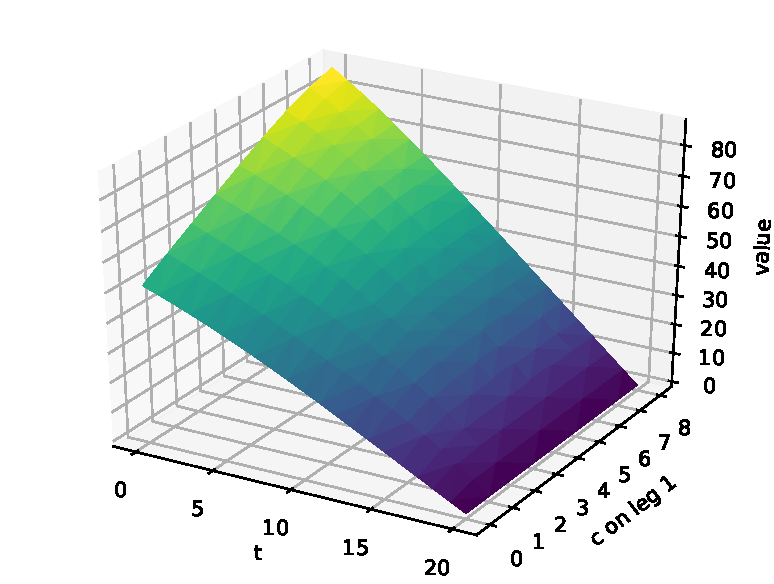
\includegraphics[width=\linewidth]{C:/Users/Stefan/LRZ Sync+Share/Masterarbeit-Klein/Code/Results/exampleStefan-True-ES-MultiLeg-190827-1516/ES-Value-c1.pdf}
		\caption{Varying capacity on leg 1.}
	\end{subfigure}
	\begin{subfigure}[b]{.49\linewidth}
		\centering
		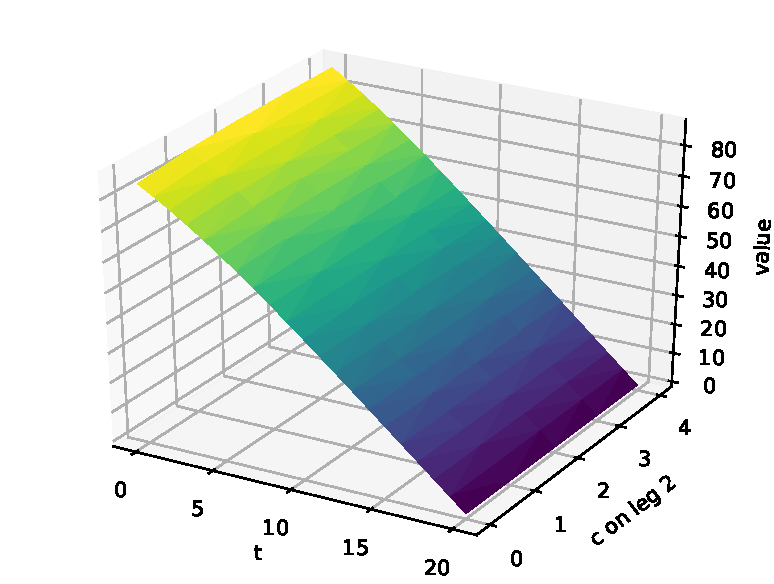
\includegraphics[width=\linewidth]{C:/Users/Stefan/LRZ Sync+Share/Masterarbeit-Klein/Code/Results/exampleStefan-True-ES-MultiLeg-190827-1516/ES-Value-c2.pdf}
		\caption{Varying capacity on leg 2.}
	\end{subfigure}
	\begin{subfigure}[b]{.49\linewidth}
		\centering
		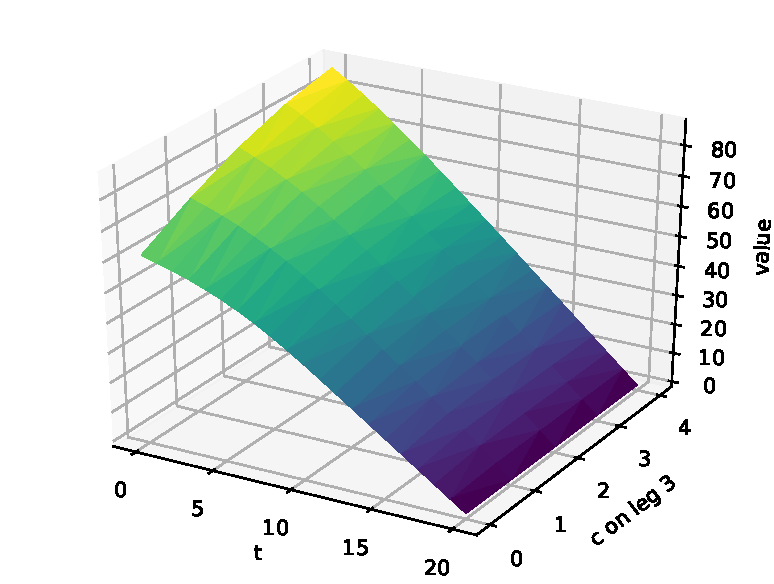
\includegraphics[width=\linewidth]{C:/Users/Stefan/LRZ Sync+Share/Masterarbeit-Klein/Code/Results/exampleStefan-True-ES-MultiLeg-190827-1516/ES-Value-c3.pdf}
		\caption{Varying capacity on leg 3.}
	\end{subfigure}
	\begin{subfigure}[b]{.49\linewidth}
		\centering
		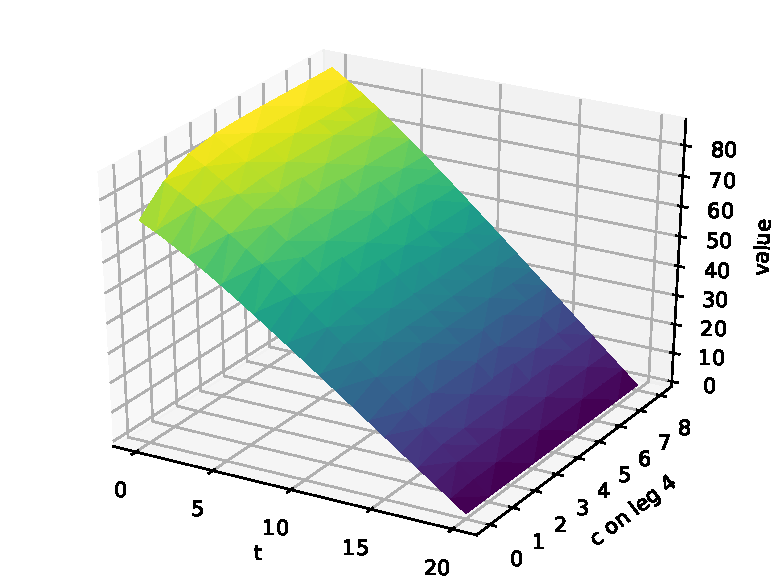
\includegraphics[width=\linewidth]{C:/Users/Stefan/LRZ Sync+Share/Masterarbeit-Klein/Code/Results/exampleStefan-True-ES-MultiLeg-190827-1516/ES-Value-c4.pdf}
		\caption{Varying capacity on leg 4.}
	\end{subfigure}
\end{figure}


Two issues make ES difficult in practice as pointed out e.g. in \cite{Koch.2017}. First, the decision problem inherent at each state (time period $t$ together with capacity $\boldsymbol{c}$) is an assortment optimization problem over $2^n$ possible offer sets. 
\todo{Ergänze Machbarkeitsanalyse in Tabellenform (Speicherbedarf plus Rechenzeit), s. hierzu VL-Unterlagen Künstl. Intelligenz}
So our small example given by \Cref{tb:AirDesc:Prod} leads to $2^6 = 64$ offer sets.
\todo{Kann das im Cache gespeichert werden (Python und Betriebssystem)}
Second, for each time period $t$, the value function \Cref{eq:Bellman} has to be computed for all possible capacities, which becomes computationally cumbersome due to multi-dimensionality ($m$ resources). In general, $\prod_{h \in [m]} (c^0_h+1)$ instances have to be solved\footnote{The capacity of each resources can take values in $\{0, 1, \dots, c^0_h\}$}. Already our small example given by \Cref{tb:AirDesc:Res} leads to a total of $9\cdot 5\cdot 5\cdot 9 = 2.025$ instances.


\subsection{Choice based linear programming}

\subsubsection{CDLP Model and direct implementation}

Because of the challenges for the exact solution as stated above, approximations are needed to solve \Cref{eq:Bellman}. A popular approach is to approximate the stochastic quantities (purchase probabilities) by deterministic values such as their expected value and to allow capacity and demand to be continuous. This approach is named \emph{Choice based linear programming} (CDLP\nomenclature{CDLP}{choice-based linear program}) and is used by e.g. \cite{GGallego.}, \cite{Liu.2008} or \cite{Bront.2009}.

Taking an eagle-eye perspective, the company has to decide which sets to offer in every single time period. But as purchase probabilities don't change over time, the specific time period when to offer an individual set is indistinguishable, we can aggregate over time. We introduce a few more notation to get a hand on this and keep it close to what is established in the literature. As already stated in \Cref{sss:DCM}, $p_{\boldsymbol{x}}(j)$ can be interpreted as the deterministic quantity of product $j$ being sold in one time period. Let $R(\mathbf{x})$ represent the expected (thus deterministic) revenue given offer set $\boldsymbol{x}$ (again per time period), and let $\boldsymbol{Q}(\boldsymbol{x}) = (Q_1(\boldsymbol{x}), \dots, Q_m(\boldsymbol{x}))^T$ denote the expected capacity being used (per time period), i.e.

\todo{Layout: Satzzeichen (Punkt oder Komma) ans Ende der Formeln mit einheitlichem Abstand}
\begin{align}
R(\boldsymbol{x}) &= \sum_{j \in [n]} r_j p_{\boldsymbol{x}}(j)\\
Q_h(\boldsymbol{x}) &= \sum_{j \in [n]} a_{hj} p_{\boldsymbol{x}}(j) \quad \forall h \in [m]\quad.
\end{align}

We can denote the total time\footnote{Total time meaning number of time periods.} for which set $\boldsymbol{x}$ is offered by $t(\boldsymbol{x})$ and the set of all possible offersets as $N = \{0,1\}^n$ . Thus, we can formulate the choice-based linear program $V^{CDLP}(T, \boldsymbol{c})$\footnote{Note that in our formulation, $p_{\boldsymbol{x}}(j)$ already includes the parameter for the arrival rate $\lambda$ and thus, $\lambda$ doesn't appear directly in our formulation of the CDLP in contrast to the fomulation in \cite{Bront.2009}.}. Here, the optimization problem is solved by varying the decision variables $t(\boldsymbol{x})$. 

\begin{align}
V^{CDLP}(T, \boldsymbol{c}): \qquad\qquad & \max \sum_{\boldsymbol{x}\in N} R(\boldsymbol{x}) t(\boldsymbol{x})\label{eq:CDLP}\\
\text{s.t. } & \sum_{\boldsymbol{x}\in N} Q_h(\boldsymbol{x}) t(\boldsymbol{x}) \leq c_h \quad, \forall h \in [m]\label{eq:CDLP-m}\\
& \sum_{\boldsymbol{x}\in N} t(\boldsymbol{x}) \leq T~,\label{eq:CDLP-1}\\
& t(\boldsymbol{x}) \geq 0 \quad \forall \boldsymbol{x} \in N~.
\end{align}

We want to mention some characteristics of this optimization problem. By allowing $t(\boldsymbol{x})$ to be continuous\footnote{E.g., $t(\boldsymbol{x})=1.2$ corresponds to offerset $\boldsymbol{x}$ being offered for one whole time period and $20\%$ of another time period.}, we arrive at a classical linear program (LP\nomenclature{LP}{linear program}), for which efficient solution methods exist (such as Simplex) and \todo{Sprache: Hier bezieht sich implemented auf die eben eingeführten solution methods} are implemented (e.g. in Gurobi). Even though the number of variables is exponential ($2^n$ as $N = \{0,1\}^n$), methods such as column-generation techniques can be used to solve this LP efficiently as \cite{GGallego.} and \cite{Liu.2008} show\footnote{Note that Gurobi is high-level and thus programmed in such way so that it realizes which method shall be used to solve a given LP efficiently.}\todo{Verify Gurobi being high-level}. Also note that the optimization problem $V^{CDLP}(T, \boldsymbol{c})$ has $m+1$ constraints ($m$ in \Cref{eq:CDLP-m} and $1$ in \Cref{eq:CDLP-1}). By duality theory and especially Complementary Slackness (compare e.g. to \cite{Domschke.2015}), at most $m+1$ basic variables will end up being non-zero. Hence, even though the number of variables being exponentially large ($2^n$), only a linear number ($m+1$) will make up \todo{Sprache: make up}the solution, which again motivates to use column-generation techniques.

The dual of the CDLP is given by
\begin{align}
	VD^{CDLP}(T, \boldsymbol{c}): \qquad \min &\boldsymbol{\pi}^T \boldsymbol{c} + \sigma T\\
	\text{s.t.} &\boldsymbol{\pi}^T \boldsymbol{Q}(\boldsymbol{x}) + \sigma \geq R(\boldsymbol{x}) \quad \forall \boldsymbol{x}\in N\\
	& \boldsymbol{\pi} \geq 0\\
	& \sigma \geq 0 ~,
\end{align}
where $\boldsymbol{\pi} \in \mathbb{R}^m$ is the vector of dual prices corresponding to the resource constraints \Cref{eq:CDLP-m} and $\sigma$ is the dual price corresponding to the time constraint \Cref{eq:CDLP-1}. Again with theory of duality in mind, the optimal value of $\pi_h$ estimates the marginal value of resource $h$ and the optimal value of $\sigma \in \mathbb{R}$ provides a marginal value of time (i.e. one additional time period would lead to an expected increase in revenue of $\sigma$ units).

In our small example, there are $256 = 2^8$ offersets and the optimal solution is presented in \Cref{txt-CDLP-Stefan}.

\begin{figure}[ht]
	\caption{Optimal solution with the null set present at start.\label{txt-CDLP-Stefan}}
	\verbatiminput{"C:/Users/Stefan/LRZ Sync+Share/Masterarbeit-Klein/Code/Results/exampleStefan-True-CDLP-190902-1649/CDLP-with-NullSet.txt"}
\end{figure}


\subsection{Solving CDLP by Column Generation}

The huge problem size, note again the $2^n$ primal variables in \Cref{eq:CDLP} might cause problems, but can be taken care of by column generation techniques as suggested by \cite{GGallego.} and pointed out by \cite{Bront.2009}. We first sketch the algorithm, then elaborate on its complexity and finally present approaches for solving the problem.

\subsubsection{CDLP Column Generation Algorithm}

The idea of handling the exponential problem size lies in starting with a small number (e.g. one) of initial offer tuples and incrementally add promising offer tuples in a clever way. We start with one offer tuple\footnote{In alignment with \cite{Bront.2009}, this offerset comprises the first product of interest of each customer segment.}, i.e. only one primal variable and solve a reduced linear program using only this column. After checking for the existence of any other offersets with positive reduced cost relative to the current dual prices of the reduced problem, we add a corresponding positive reduced cost primal variable and re-optimize the LP. If no offerset with positive reduced cost exists, the current solution of the problem is optimal.

\todo{Fußnoten checken, kommen hinter die Satzzeichen, falls sie sich auf ganzen Satz beziehen}
\todo{mathbf ersetzen durch boldsymbol}
The reduced primal CDLP problem at step \emph{k}, i.e. with $k$ offersets given by the set $\mathcal{N}=\{\mathbf{x}_1, \dots, \mathbf{x}_k\}$, is given by

\begin{align}
V^{CDLP-R}(T, \boldsymbol{c}): \qquad\qquad & \max \sum_{\boldsymbol{x}\in \mathcal{N}} R(\boldsymbol{x}) t(\boldsymbol{x})\label{eq:CDLPr}\\
\text{s.t. } & \sum_{\boldsymbol{x}\in \mathcal{N}} Q_h(\boldsymbol{x}) t(\boldsymbol{x}) \leq c_h \quad, \forall h \in [m]\\
& \sum_{\boldsymbol{x}\in \mathcal{N}} t(\boldsymbol{x}) \leq T~,\\
& t(\boldsymbol{x}) \geq 0 \quad \forall \boldsymbol{x} \in \mathcal{N}~.
\end{align}

Again, with $\boldsymbol{\pi} \in \mathbb{R}^m$, resp. $\sigma \in \mathbb{R}$ denoting the dual prices of resources, resp. time, the corresponding dual problem is given by

\begin{align}
VD^{CDLP-R}(T, \boldsymbol{c}): \qquad \min &\boldsymbol{\pi}^T \boldsymbol{c} + \sigma T\label{eq-CDLPr}\\
\text{s.t.} &\boldsymbol{\pi}^T \boldsymbol{Q}(\boldsymbol{x}) + \sigma \geq R(\boldsymbol{x}) \quad \forall \boldsymbol{x}\in \mathcal{N}\label{eq-CDLPr-col}\\
& \boldsymbol{\pi} \geq 0\\
& \sigma \geq 0 ~.
\end{align}

\todo{Theory on reduced costs and column generation, why do we look for primal variables with positive reduced costs?}

Let us analyse $V^{CDLP-R}(T, \boldsymbol{c})$ in more depth to explore the ideas behind column generation algorithms. \Cref{eq-CDLPr} shall be minimized by altering the (dual) variables $\boldsymbol{\pi}$ and $\sigma$. These variables are bounded from below by $0$ and have to satisfy \Cref{eq-CDLPr-col}. At this point, we introduce the reduced costs of an offerset $\boldsymbol{x}$ as $rc(\boldsymbol{x}) \coloneqq R(\boldsymbol{x}) - \boldsymbol{\pi}^T \boldsymbol{Q}(\boldsymbol{x}) - \sigma$ and realize that \Cref{eq-CDLPr-col} is equivalent to $rc(\boldsymbol{x}) \leq 0$, i.e. all offersets in $\mathcal{N}$ are ensured to have negative reduced costs (the dual variables are chosen in such manner). Remember $N = {0, 1}^n$, thus we skipped all offersets $\boldsymbol{x} \in N \backslash \mathcal{N}$. If an offerset $\hat{\boldsymbol{x}}$ has negative reduced costs, adding $\hat{\boldsymbol{x}}$ to $\mathcal{N}$ results in one additional constraint in \Cref{eq-CDLPr-col}, which is inactive, i.e. satisfied (we added variable $\hat{\boldsymbol{x}}$ with negative reduced costs). Thus, the objective value wouldn't change as the additional constraint doesn't put a restriction on the optimal dual variables $\boldsymbol{\pi}$ and $\sigma$. In the contrary, when considering an offerset $\check{\boldsymbol{x}}$ with positive reduced costs, adding the corresponding constraint in the dual problem results in a violation of \Cref{eq-CDLPr-col}. Thus, the corresponding constraint is active and $\boldsymbol{\pi}$ and $\sigma$ have to be adjusted to become admissible again. 

Having this idea in mind motivates the column generation subproblem:\footnote{Note that in comparison to \cite{Bront.2009}, the potential offersets to consider can be limited to $N \backslash \mathcal{N}$ as $\boldsymbol{\pi}$ and $\sigma$ are chosen in such manner that $rc(\boldsymbol{x}) \leq 0$ is ensured $\forall \boldsymbol{x}\in \mathcal{N}$.}

\begin{align}
	\max_{\boldsymbol{x} \in N} rc(\boldsymbol{x}) = \max_{\boldsymbol{x} \in N} \{R(\boldsymbol{x}) - \boldsymbol{\pi}^T \boldsymbol{Q}(\boldsymbol{x})\} - \sigma \label{eq-ColGen}
\end{align}

If the optimal solution to \Cref{eq-ColGen} is positive, we augment $\mathcal{N}$ with the corresponding $\hat{\boldsymbol{x}} = \argmax_{\boldsymbol{x} \in N} rc(\boldsymbol{x})$ (note once more that $rc(\hat{\boldsymbol{x}}) > 0$ and thus $\hat{\boldsymbol{x}}$ is not part of the old $\mathcal{N}$). 

If the optimal solution to \Cref{eq-ColGen} is non-positive, the current solution is already optimal. Let's elaborate on this. $V^{CDLP}(T, \boldsymbol{c})$ differs from $V^{CDLP-R}(T, \boldsymbol{c})$ only in the considered set of offersets, all $N$ versus the reduced $\mathcal{N}$. We augmented $\mathcal{N}$ to a point, when the column generation subproblem $\Cref{eq-ColGen}$ results in a non-positive solution. Now, \Cref{eq-CDLPr-col} is satisfied $\forall \boldsymbol{x} \in \mathcal{N}$ (by construction), but also $\forall \boldsymbol{x} \in N$ (compare to the optimal solution of the column generation subproblem). In summary, the optimal value of $VD^{CDLP-R}(T, \boldsymbol{c})$ equals the optimal value of $VD^{CDLP}(T, \boldsymbol{c})$. Furthermore, $VD^{CDLP}(T, \boldsymbol{c})$ equals $V^{CDLP}(T, \boldsymbol{c})$ as strong duality holds because we are dealing with a linear optimization problem and have found a feasible solution for the dual, which is a sufficient condition for strong duality as proven in Theorem $6.1.7 b)$ of \cite{Gritzmann.2013}.

Note that, up to now, we have not considered a particular customer choice model. Let us continue with introducing the MNL choice model also in this (CDLP) context, in order to analyse it's complexity in the following. With MNL as customer choice model, \Cref{eq-ColGen}  can be expressed as (all equivalent)

\begin{align}
\max_{\boldsymbol{x} \in \{0, 1\}^n}\left\{ \sum_{j \in [n]} r_j p_{\boldsymbol{x}}(j) - \sum_{h \in [m]} a_{hj} \pi_h p_{\boldsymbol{x}}(j) \right\} - \sigma\\
\max_{\boldsymbol{x} \in \{0, 1\}^n}\left\{ \sum_{j \in [n]} \left(r_j  - A_j^T\boldsymbol{\pi}\right) p_{\boldsymbol{x}}(j) \right\} - \sigma\\
\max_{\boldsymbol{x} \in \{0, 1\}^n}\left\{ \sum_{l \in [L]} \lambda_l \frac{\sum_{j \in [n]} \left(r_j  - A_j^T\boldsymbol{\pi}\right)u_{lj}x_j}{\sum_{j \in [n]} u_{lj}x_j + u_{l0}} \right\} - \sigma\\
\max_{\boldsymbol{x} \in \{0, 1\}^n}\left\{ \sum_{j \in [n]} \left(r_j  - A_j^T\boldsymbol{\pi}\right) x_j \left( \sum_{l \in [L]} \frac{\lambda_l u_{lj} }{\sum_{j \in [n]} u_{lj}x_j + u_{l0}} \right)\right\} - \sigma\label{eq-ColGen-sub}
\end{align}

Note that the assumptions $u_{lj} \in \mathbb{R}^+_0 \quad \forall j \in [n]$, resp. $u_{l0} \in \mathbb{R}^+$ ensure the optimization problem to always be well defined.

\subsubsection{Complexity of Column Generation}

As noted in \cite{Bront.2009}, \Cref{eq-ColGen-sub} is in general not separable in the variables $x_j, j\in[n]$ as multiple customer segments (e.g. $l_1$ and $l_2$) might be interested in the same product $j$ and thus, $x_j$ appears in the denominator belonging to $l_1$ and in the one belonging to $l_2$. Our column generation problem is part of the general group of \emph{hypberbolic (or fractional) 0-1 programming problems}, which were studied by e.g. \cite{Hansen.1991} or \cite{Borrero.2017} and the most general version is given by

\todo{footnote to max(x) = min(-x) even if x aus 0, 1}

\begin{align}
	\max_{\boldsymbol{x} \in \{0,1\}^n} \sum_{l \in [L]} \frac{a_{l0} + \sum_{j \in [n]}a_{lj}x_j}{b_{l0} + \sum_{j \in [n]} b_{lj}x_j}~,\label{eq-hyp}
\end{align}

\todo{Exkursion zu Komplexität, was ist NP-hard}
with no restrictions on $a_{lj}, b_{lj}$ and $x_j \in \{0, 1\} \forall j \in [n]$. \cite{Prokopyev.2005} have proven that \Cref{eq-hyp} is NP-hard by providing a polynomial reduction from the weighted 2SAT problem. 

\todo{ggf. Einschub von Ryzin and Liu (2004, §6.3.1) zu disjoint segments}

\todo{Give example on difficult linkage.}
\cite{Bront.2009} point out that due to the tight linkage of variables in our column generation subproblem, the general \Cref{eq-hyp} cannot be easily reduced to the specific \Cref{eq-ColGen-sub}. But they reduce the \emph{minimum vertex cover problem} to our problem \Cref{eq-ColGen-sub}. And as \cite{Garey.ca.2009} proofs the \emph{minimum vertex cover problem} to be NP-hard\footnote{Stated in [GT1] Vertex Cover under \emph{A1.1 Covering and Partitioning} on page 190 and referred to \cite{Karp.2010}, who proves NP-hardness by a transformation from 3SAT, the well established example for a problem of the NP-class.}, our column generation problem is NP-hard as well. 

\todo{evtl. weiter ausführen}

%\clearpage
%\setcounter{page}{1}
%\noindent\fbox{\parbox{\textwidth}{\centering 04.09.}}

\subsubsection{Approaches for solving Column Generation}

\textbf{MIP Formulation}. We follow \cite{Bront.2009} to formulate the column generation problem \Cref{eq-ColGen} as a mixed integer problem (MIP\nomenclature{MIP}{mixed integer problem}).  To get rid of the fraction, we introduce the new variable

\begin{align}
	y_l = \frac{1}{\sum_{j \in [n]} u_{lj}x_j + u_{l0}}~,
\end{align}

and enforce this via the (non-fractional) constraint in \Cref{const-frac}. By also changing the order of summation\footnote{Changing the order of summation is allowed since the sum is finite.}, using the distributive law and ignoring the constant $\sigma$ (we check if the optimal result is $> \sigma$ in the end\todo{check if optimal column generation is greater sigma}), we rewrite the column generation problem \Cref{eq-ColGen-sub} as\footnote{Note that \cite{Bront.2009} used sloppy notation by claiming $j\in N$, as she introduced $N$ to be a constant (the total number of products). Our notation is precise.}

\begin{align}
\max_{\boldsymbol{x}, \boldsymbol{y}} \sum_{l \in [L]}\sum_{j \in [n]} (r_j - A_j^T\boldsymbol{\pi}) x_j \lambda_l u_{lj} y_l\\
\text{s.t. }y_l u_{l0} + \sum_{j \in [n]} u_{lj} x_j y_l = 1 ~,\quad \forall l in [L] \label{const-frac}\\
x_j \in \{0, 1\} ~,\quad \forall j \in [n]\\
y_l \geq 0 ~,\quad \forall l \in [L]~.
\end{align}

It remains to linearise the nonlinear term (product) $x_j y_l$. We first introduce the concept of linearizing $x y$ with $x\in \{0, 1\}$ and $y \geq 0$ following \cite{Klein.2017}. We introduce the auxiliary variable $z \geq 0$. Obviously, we want $z = 0$ if $x=0$. This leads to the constraint $z \leq x y$. And we want $z = y$ if $x=1$. This can be enforced by putting the constraints $z \leq y$\footnote{Note that this constraint is already included in the previous one $z \leq y x$, thus can be excluded here. This thought can be used to enhance \cite{Klein.2017} by combining constraints (1.20) and (1.20) to $\lambda_{ij} \leq p_j x_{ij}$. Note that constraint (1.20) does not really come from enforcing the linearization, but from the participation constraint (1.14).} and $z \geq y - M(1-x)$ with $M$ large enough (this idea of introducing a large constant to switch off a constraint if need be is generally referred to as \emph{big M}). Note that the other constraints are trivially fulfilled if $x=1$, resp. $x=0$. We apply these ideas and introduce the auxiliary variable $z_{lj} = x_j y_l$ with the corresponding constraints and obtain the MIP formulation

\begin{align}
\max_{\boldsymbol{x}, \boldsymbol{y}} \sum_{l \in [L]}\sum_{j \in [n]} (r_j - A_j^T\boldsymbol{\pi}) \lambda_l u_{lj} z_{lj}\\
\text{s.t. }y_l u_{l0} + \sum_{j \in [n]} u_{lj} z_{lj} = 1 ~,\quad \forall l \in [L] \label{const-frac}\\
y_l - z_{lj} \leq M(1-x_j) ~,\quad \forall l\in [L]\forall j \in [n]\label{M}\\
z_{lj} \leq y_l x_j ~,\quad \forall l\in [L]\forall j \in [n]\label{z}\\
x_j \in \{0, 1\} ~,\quad \forall j \in [n]\\
y_l \geq 0 ~,\quad \forall l \in [L]\\
z_{lj} \geq 0 ~,\quad \forall l\in [L]\forall j \in [n]~,
\end{align}

with $M \geq 1/\min\{u_{l0}: l\in [L]\}$\footnote{In comparison to \cite{Bront.2009}, we adopt the minimum as not all products might be in the consideration set, thus $\underline{v}$ might be $0$. Our denominator will always be nonzero, as all $u_{l0}$ are assumed to be $>0$, and will be appropriate as potentially adding some positive $u_{lj}$ just increases the denominator, thus decreases $M$.}. $M$ is large enough, because \Cref{M} is satisfied if activated ($x_j = 0$) as $z_{lj}$ is then forced to zero by \Cref{z} and $y_l$ potentially set to $1/u_{l0}$ by \Cref{const-frac}. 

Having such a MIP formulation allows for the usage of standard MIP solvers like Gurobi. But as the complexity result of \cite{Bront.2009} states, the column generation problem is still NP hard. Thus, we present a polynomial time heuristic.

\textbf{Greedy Heuristic} 

We use a greedy, constructive heuristic as suggested by \cite{Bront.2009} and adopt notation. The algorithm was already proposed by \cite{Prokopyev.2005b} to solve a general fractional programming problem and makes a straightforward use of the most promising offersets. It aims at constructing the most promising offerset to add to the sets of offersets $\mathcal{N}$. Note that, via the current $\mathcal{N}$, we arrived at the values of the dual variables $\boldsymbol{\pi}$ and $\sigma$. The algorithm starts in \Cref{alg-CG-1} with defining the set $S'$ of promising products, i.e. such products with positive reduced costs. \Cref{alg-CG-2} really just rewrites the column generation subproblem \Cref{eq-ColGen-sub} by summing solely over the products to select instead of summing over all products and just keeping those for which $x_j=1$. The most promising product $j^*$ is selected and set $S$ keeps track of all selected products. More products are selected as long as this results in an increase of value for the objective function $f$. The heuristic itself is given by the following\footnote{Note that our first $j^*$ is found in \Cref{alg-CG-3} in consistence with the other $j^*$'s found in \Cref{alg-CG-6}, i.e. including the arrival probabilities $\lambda_l$. This is not the case in \cite{Bront.2009}, compare step 3 with step 4.a.}.

\begin{algorithm}
	\caption{Heuristic for column generation}\label{alg-ColGen}
	\begin{algorithmic}[1]
		\State Define $S \coloneqq \emptyset$ and $S^{'} \coloneqq \{j \in [n]: r_j - A_j^T\boldsymbol{\pi} > 0\} \subset [n]$ \label{alg-CG-1}
		\State Define $f(S') \coloneqq \max_{j \in S^{'}} \sum_{l \in [L]} \lambda_l  \frac{\sum_{p \in S \cup \{j\}} (r_p - A_p^T\boldsymbol{\pi}) u_{lp}}{\sum_{p \in S \cup \{j\}}u_{lp} + u_{l0}}\label{alg-CG-2}$
		\State Compute $ j^* = \arg \max_{j \in S'} f(S') \label{alg-CG-3}$
		\State Set $S \coloneqq \{j^*\}, S^{'} \coloneqq S' \backslash \{ j^*\}$
		\Repeat
			\State Compute $ j^* = \arg \max_{j \in S'} f(S') \label{alg-CG-6}$
			\If{$f(S \cup \{j^*\}) > f(S)$}
			\State Set $S \coloneqq S \cup \{j^*\}, S^{'} \coloneqq S' \backslash \{ j^*\}$
			\EndIf
		\Until $S$ is not modified
		\State \Return Offerset $\boldsymbol{x}$ given by $x_j = \mathbbm{1}_{\{j \in S\}}, ~j\in[n]$
	\end{algorithmic}
\end{algorithm}

This heuristic has worst-case complexity of $O (n^2 L)$ as the repeat loop might run for all $n$ products and in \Cref{alg-CG-6} the calculation of the argmax of $f$ is done $\abs{S'}$ times with a summation over all $L$ customer segments and the remaining, $n - \abs{S'}$ products. Note that in practice, there are much less customer segments than products, i.e. $L << n$.

Furthermore, we want to mention an adopted version\footnote{We adjust the parameters $\lambda_l = 1/3$ so that they sum up to $1$. Note that this is necessary due to our assumption of at most one customer arriving at a given point in time. To reproduce the optimal values stated in \cite{Bront.2009}, we just have to multiply by $3$ due to the scalability of Poisson processes as stated in .}\todo{add link to proof Poisson processes} of the example in $\cite{Bront.2009}$, which shows that \Cref{alg-ColGen} is indeed a heuristic, i.e. stops without finding the optimal solution. We also use this example for a first validation of our code. Consider the column generation subproblem \Cref{eq-ColGen-sub} with $n=3, L=3$, the other values as specified in \Cref{fig-ColGen} and $\boldsymbol{\pi} = (0, 0, 0)^T$. Applying our implemented functions result in \Cref{txt-CDLP-Greedy}, which proofs that the greedy heuristic was unable to find the optimum as it stopped at the optimal value of $16.66$ instead of arriving at the truly optimal $17.83$.

\begin{figure}
	\caption{Small example for illustration of sub-optimality of CDLP Greedy Heuristic with $T=1$ time period.\label{fig-ColGen}}
	\begin{subfigure}[t]{.3\linewidth}
		\centering
		\caption{Airline network.}
		\begin{tikzpicture}[
		mycircle/.style={
			circle,
			draw=black,
			fill=gray,
			fill opacity = 0.3,
			text opacity=1,
			inner sep=0pt,
			minimum size=20pt,
			font=\small},
		myarrow/.style={-Stealth},
		node distance=0.6cm and 1.2cm
		]
		\node[mycircle] (cA) {$A$};
		\node[mycircle,right=of cA] (cB) {$B$};
		
		\draw[myarrow](cA) -- node[sloped,font=\small,above] {Leg 1} (cB);
		\end{tikzpicture}
	\end{subfigure}%
	\quad
	\begin{subtable}[t]{.4\linewidth}
		\caption{Products. }
		\small
		\centering
		\begin{tabular}{yxz}
			\toprule
			\text{Product} & \text{Origin-destination} & \text{Fare}\\
			\midrule
			1 & A \rightarrow B & 100\\
			2 & A \rightarrow B & 19\\
			3 & A \rightarrow B & 19\\
			\bottomrule
		\end{tabular}
	\end{subtable}%
	\quad
	\begin{subtable}[t]{.2\linewidth}
		\caption{Resources. \label{tb:AirDesc:Res}}
		\small
		\centering
		\begin{tabular}{yy}
			\toprule
			\text{Leg} & \text{Capacity}\\
			\midrule
			1 & \infty\\
			\bottomrule
		\end{tabular}
	\end{subtable}
	
	\begin{subtable}{\linewidth}
		\caption{Customers.\label{tb:AirDesc:Cust}}
		\small
		\centering
		\begin{tabular}{lccccc}
			\toprule
			Seg. & $\lambda_l$ & \specialcell[b]{Consideration\\tuple} & \specialcell[b]{Preference \\vector} & \specialcell[b]{No purchase \\preference} & Description\\
			\midrule
			1 & $1/3$ & $(1, 2, 3)$ & $(1, 1, 1)$ & $1$ & Flexible, (A$\rightarrow$B)\\
			2 & $1/3$ & $(2)$ & $(1)$ & $1$ & Just $2$, (A$\rightarrow$B)\\
			3 & $1/3$ & $(3)$ & $(1)$ & $1$ & Just $3$, (A$\rightarrow$B)\\
			\bottomrule
		\end{tabular}
	\end{subtable}
\end{figure}

\begin{figure}[ht]
	\caption{Results for example of greedy heuristic.\label{txt-CDLP-Greedy}}
	\verbatiminput{"C:/Users/Stefan/LRZ Sync+Share/Masterarbeit-Klein/Code/Results/exampleGreedy-True-CDLP-190904-1355/CDLP-exampleGreedy.txt"}
\end{figure}

\vspace*{1cm}
\noindent\fbox{%
	\parbox{\textwidth}{%
		Our implementation of the CDLP by column generation consists of: First, we use the greedy heuristic to identify a promising offerset. If this method doesn't succeed, we use the exact MIP procedure. If no new offerset is identified to enter the base, we have found the optimal solution of the CDLP.%
	}%
}
\vspace*{1cm}

Applying this version of CDLP by column generation to our running Example, we find \Cref{txt-CDLP-ColGen-Stefan}. Note that the same solution is found as by using CDLP, compare to \Cref{txt-CDLP-Stefan}. But the column generation algorithm needs just $3$ columns in comparison to $256$ used by CDLP.

\begin{figure}[ht]
	\caption{Optimal solution for CDLP by column generation for running example.\label{txt-CDLP-ColGen-Stefan}}
	\verbatiminput{"C:/Users/Stefan/LRZ Sync+Share/Masterarbeit-Klein/Code/Results/exampleStefan-True-CDLP-190904-1432/CDLP-columnGeneration.txt"}
\end{figure}


\section{Approximate Dynamic Programming}

ADP builds upon \Cref{eq:DP-optOffer}. The real challenge lies in determining the opportunity costs $\Delta_j V(t+1, \boldsymbol{c})$. ADP approximates these opportunity costs additively using bid prices $\pi_h(t, c_h)$, i.e. $\Delta_j V(t+1, \boldsymbol{c}) = \sum_{h \in [m]} a_{hj}\pi_{h}(t+1, c_h)$. Thus, the policy is given as the solution of

\begin{align}
^\pi \boldsymbol{x}^t = \argmax_{x^t \in \{0,1\}^n}\left\{ \sum_{j \in [n]} p_j(x_t) \left( r_j - \sum_{h \in [m]} a_{hj}\pi_{h}(t+1, c_h) \right) \right\}~,\label{eq:ADP-online}
\end{align}

and is therefore completely described by the bid prices $\pi_h(t, c_h) \forall t \in [T]$. Note that $\boldsymbol{x}^t$ represents the set offered during time period $t$, i.e. the decision is made at time point $t-1$ and $\Delta_j V(t+1, \boldsymbol{c})$ represents the difference in revenue to go when looking at product $j$ and considering time periods $t+1, \dots, T$ and capacity $c_h$.

We now present a brief overview how to classify simulation based ADP methods, which is dealt with in more detail in the textbook of \cite{Bertsekas.2005} or \cite{Powell.2011}. The methods are named \emph{approximate}, as they are based on approximating the value function. Various sample paths are generated and used in basically two different manners to iteratively improve the approximation of the value function: either by approximate value iteration (AVI\nomenclature{AVI}{approximate value iteration}) or by approximate policy iteration (API). Each iteration of AVI comprises a single sample path. It evaluates the current policy on this particular sample path and updates parameters for the value function approximation after each period of the sample path. In contrary, each iteration of API  comprises multiple sample paths. It evaluates the current policy on a set of sample paths and uses the combined information to update and improve the value function approximation (and thus the policy). Thus, one iteration of API is certainly costlier and usually API requires less iterations to obtain good policies. One obvious prerequisite for this is a large enough set of sample paths and we refer to \cite{Powell.2011} for more details.

The method proposed by \cite{Koch.2017} belongs to the class of simulation based ADP. More precisely, it comprises a value function approximation algorithm and uses policy iteration. It approximates the value function $V(t, \boldsymbol{c})$ by computationally simple functions (linear or piecewise linear). It makes use of an offline phase to determine bid prices $\pi_h(t, c_h) \forall t \in [T]$ (for each time period) and applies \Cref{eq:ADP-online} in an online phase to present the offerset.

\subsection{Approximate Policy Iteration}

Approximate Policy Iteration is used in the offline phase and aims at determining bid prices for each time period $\pi_h(t, c_h) \forall t \in [T]$, which fully determine the policy used in the online phase. The complete algorithm is given by \Cref{alg-API} and comprises several steps. We first give an overview of the concept and then start from the inside and work our way outwards.

\subsubsection{API value function approximation}

As there are quite some variables involved in API, we created \Cref{tb-api-param} for reference. We will introduce the concept of the method in the following.

\begin{table}
	\caption{API Overview of parameters.\label{tb-api-param}}
	\begin{tabular}{ll}
		$\theta_t$ & optimization parameter (offset)\\
		$\boldsymbol{\pi}_t$ & optimization parameter (bid price for each resource)\\
		$\hat{V}_t $ & all sample revenues to go for each sample for each time period\\
		$\boldsymbol{\hat{C}}_t$ & all sample available capacities for each sample for each resource for each time period\\
		$r_t$ & sample revenue generated during time period $t$\\
		$\boldsymbol{c}$ & available capacities for each resource at current time period\\
		$\boldsymbol{c}^0$ & starting capacities\\
		$\boldsymbol{x}$ & offerset at current time period\\
		$\epsilon_t$ & epsilon used at current time period
	\end{tabular}
\end{table}

API aims at approximating the value function. As a state is characterized by current time period $t$ and vector of current capacities $\boldsymbol{c}$, a natural choice is to use a linear function as given by

\begin{align}
V_{t,\boldsymbol{c}}(\theta_t, \boldsymbol{\pi}_t) \coloneqq \theta_t + \sum_{h \in [m]} \pi_{th} c_h\\
\text{with}\\
\theta_t \geq 0\label{eq-api-theta}\\
\max_{j=1, \dots, n} r_j \geq \pi_{th} \geq 0\label{eq-api-pi}
\end{align}

\todo{graph: Add graph, why the two other constraints are necessary}
and $\theta_{T+1} = 0$ as well as $\pi_{T+1, h} = 0 \forall h\in[m]$ assumed implicitly ($V(T+1, \boldsymbol{c}) = 0 if \boldsymbol{c} \geq \boldsymbol{0}$). Note that we follow \cite{Koch.2017} and include expert knowledge on the problem. The non-negativity constraints in \Cref{eq-api-theta} and \Cref{eq-api-pi} ensure that the optimal value is non-negative and increasing in capacity. The upper bound in \Cref{eq-api-pi} is also reasonable as one additional capacity should increase the optimal value less than the most expensive product. This directly leads us to the interpretation of the constraints. $\theta_t$ represents the constant offset. $\pi_{th}$ can be directly interpreted as bid prices of the resources, and therefore be used in \Cref{eq:ADP-online}:  $\pi_h(t+1, c_h) = \pi_{th}$. Note that in this setting, the bid price is independent of the current level of capacity.

\subsubsection{API overview}

\begin{algorithm}
	\caption{Approximate policy iteration. Note that $t$ almost always represents time period and therefore takes values in $\{1, \dots, T\}$. As at time period $t$, there is $c_{t-1}$ capacity available, we use a different index for capacity.}\label{alg-API}
	\begin{algorithmic}[1]
		\State Set $\theta_t = 0$ and $\boldsymbol{\pi}_t = \boldsymbol{0}$ $\forall t \in [T]$ \label{alg-API1}
		\For{\texttt{k = 1 to K}} \label{alg-API-Piter1}
		\State Set $\hat{V}_t^i = 0$ and $\boldsymbol{\hat{C}}_{t-1}^i = 0$ $\forall t \in [T], \forall i \in [I] $ \label{alg-API-Piter2}\label{alg-API3}
		\For{\texttt{i = 1 to I}}\label{alg-API-Peval1}
		\State Set $\hat{r}_t = 0$ and $\boldsymbol{\hat{c}}_{t-1} = 0$ $\forall t \in [T]$ \label{alg-API5}
		\State Initialize $\boldsymbol{c} = \boldsymbol{c}^0$\label{alg-API6}
		\For{\texttt{t = 1 to T}}
		\State $\boldsymbol{\hat{c}}_{t-1} \coloneqq \boldsymbol{c}$\label{alg-API8}
		\State Assign $\boldsymbol{\pi}(t, \boldsymbol{c})$ \label{alg-API-calcPi}\label{alg-API9}
		\State Compute $\boldsymbol{x} = \text{determineOfferset}(\boldsymbol{\pi}(t, \boldsymbol{c}), \epsilon_t)$ \label{alg-API10}
		\State Simulate a sales event $j' \in \{0, 1, \dots, n\}$\label{alg-API11}
		\If{$j' \in \{ 1, \dots, n\}$}
		\State $\hat{r}_t = r_{j'}$ and $\boldsymbol{c} = \boldsymbol{c} - \boldsymbol{a}_{j'}$\label{alg-API13}
		\EndIf
		\EndFor
		\State Compute $\hat{V}_t^i = \sum_{\tau = t}^{T}\hat{r}_t \quad \forall t \in [T]$\label{alg-API14}
		\State Assign $\boldsymbol{\hat{C}}_{t-1}^i = \boldsymbol{\hat{c}}_{t-1} \quad \forall t \in [T]$ \label{alg-API15} \label{alg-API-Peval2}
		\EndFor
		\State $\left(\theta_t, \pi_t \right) = \text{updateParameters}\left(\hat{V}_t^i, \boldsymbol{\hat{C}}_{t-1}^i, \theta_t, \pi_t, k\right) \quad \forall t \in [T], \forall i \in [I]$ \label{alg-API-updateParam}\label{alg-API-Piter3}
		\EndFor
		\Return {$\left(\theta_t, \pi_t \right)  \quad \forall t \in [T]$}
	\end{algorithmic}
\end{algorithm}

Let us now discuss the algorithm in depth.\footnote{We strictly use our notion of time periods in this thesis. Note that there is a one on one correspondence of \enquote{action happening during time period $t$ with $t\in[T]$} and \enquote{action happening at time point $t$ with $t\in \{0, \dots, T-1\}$}. The latter is more convenient to use in the Python implementation as Python indexing starts at $0$.} In the beginning (\Cref{alg-API1}), all parameters are set to zero which results in the greedy policy of simply offering the set resulting in the highest expected revenue (no consideration of costs) in each time period.

Then, a total of $K$ policy iterations follow.\footnote{Note that this direct approach is used in \cite{Koch.2017}. While $K$ was presumably found looking at convergence rates and then fixed, I would encourage practitioners to directly apply a convergence criterion for termination of policy iteration. Note that policy iteration is proven to converge if we added a discounting factor of later revenues to our setting. Compare \cite[Proposition 1.3.6 on p. 48]{Bertsekas.2005}.} In each policy iteration $k$, the current policy is evaluated first. To do so, we use the current policy to evaluate $I$ random sample paths. \Cref{alg-API3} sets up the dataset for revenues to go $\hat{V}_t^i$ and remaining capacities $\boldsymbol{\hat{C}}_{t-1}^i$ for all time periods $t \in [T]$ and sample paths $i \in [I]$. 

For each sample path $i$, a storage unit for revenue $\hat{r}_t$ is created for all time periods $t \in [T]$ and all capacities $\boldsymbol{\hat{c}}_{t-1}$ (\Cref{alg-API5}). Note, that we use a different index for capacities to account for the fact that for the remaining revenues to go starting from and including time period $t$, we have capacities $\boldsymbol{c}_{t-1}$ available (those being left over from time period $t-1$.). Furthermore, the capacity is set to the initial capacity in \Cref{alg-API6}.

For each time period, the available capacity $\boldsymbol{\hat{c}}_{t-1}$ (left over at end of previous time period) is stored in \Cref{alg-API8}, the current bid prices are calculated in \Cref{alg-API9} and used to determine the offerset $\boldsymbol{x}$ in \Cref{alg-API10}. More details on the determination of the offerset can be found in \Cref{sec-determineOfferset}. With, this, a sales event $j'$ is simulated and in case a product has been sold, the revenue is stored and capacity adjusted accordingly (note: the revenue thus belongs to time period $t$ and capacity will affect time period $t+1$) (\Cref{alg-API11} to \Cref{alg-API13}).

After simulating one sample path, the value function for this sample path $\hat{V}_t$ is computed for all time periods $t\in[T]$ in \Cref{alg-API14}, and so are the capacities in \Cref{alg-API15}.

Before expanding on how the parameters $\theta, \boldsymbol{\pi}$ are updated, we want to fill the gap on how the offerset is determined in \Cref{alg-API10}.

\subsubsection{API determination of offersets}\label{sec-determineOfferset}

Our goal is to determine a reasonable set of products to offer in a fast manner. Thus, we use a heuristic and cut down the amount of products to consider as fast as possible. The following algorithm is based on the ideas of the greedy, largest marginal benefit heuristic for the column generation subproblem outlined in \cite{Bront.2009} and above \todo{combine and explain just once}.

%todo expand on exploration vs exploitation dilemma
The function $\texttt{determineOfferset}(\boldsymbol{\pi}, \epsilon)$ calculates the set to offer depending on the current bid prices $\boldsymbol{\pi}$ via the greedy algorithm pointed out in \cite{Bront.2009}. As we put ourselves into a policy improvement setting and started out with the greedy strategy, the whole procedure tends to find solely other policies rather closeby, i.e. also greedy. Thus, we would leave out a big portion of the whole solution space (for each time period and each combination of capacities any subset of the $n$ products can be offered). This is the famous exploration vs. exploitation dilemma. The current solution was found and improved already and should be exploited further (comparable to incremental innovation), but also other parts of the solution space should be explored (comparable to disruptive innovation). To account for this dilemma, we follow \cite{Koch.2017} and use an epsilon-greedy strategy. With a probability of $\epsilon/2$ either no product is offered at all or all products with positive contribution $r_j - \sum_{h \in [m]} a_{hj} \cdot \pi_h$ are offered. With a probability of $1-\epsilon$, the set determined by \Cref{alg-GreedyHeuristic} is offered.

\begin{algorithm}
	\caption{Greedy Heuristic}\label{alg-GreedyHeuristic}
	\begin{algorithmic}[1] % [1] results in line numbers
		% Großes X verwendet, um Menge zu symbolisieren
		\State $\text{Value}(X) \coloneqq \sum_{l=1}^{L} \lambda_l \frac{\sum_{i \in X}(r_i - A_i^T\pi)u_{li}}{\sum_{i \in X}u_{li} + u_{l0}}$
		\State $S\coloneqq \emptyset,\quad S' \coloneqq \left\{j \in N : r_j - A_j^T\pi > 0\right\}$ \label{alg-L1}
		\State $j^* \coloneqq \arg\max_{j \in S'} \text{Value}(\{j\})$
		\Repeat
		\State $S \coloneqq S \cup \{j^*\},\quad S' \coloneqq S'\backslash\{j^*\}$
		\State $j^* \coloneqq \arg \max_{j \in S'} \text{Value}(S \cup \{j\})$
		\Until {$\text{Value}(S \cup \{j^*\}) \leq \text{Value}(S)$\\}
		\Return {$S$}
	\end{algorithmic}
\end{algorithm}

Note that in the very first iteration, we do not have appropiate values for $\boldsymbol{\pi}$ and $\theta$. Thus, we decided to set them to zero at start, corresponding to \enquote{no opportunity costs of resources}.


\subsubsection{API update of parameters}\label{sec-updateParameter}

With the information of the $I$ sample paths, the parameters $\left(\theta_t, \boldsymbol{\pi}_t \right)$ are updated. Note that the old parameters are used as starting values and the current number of policy iterations $k$ is also passed to potentially take care of exponential smoothing. Thus, we have $(1+h)*T$ parameters ($\theta_t$ and $\boldsymbol{\pi}_t$) and $TI$ data points (each data point comprises the value of the value function as $y$-value and the current assignment of $t$ and $\boldsymbol{\pi}_t$ as $x$-values). 


$\Theta, \Pi, C$

\todo{Schreibweise der Funktion anpassen, da alle Parameter auf einmal übergeben werden, und nicht separat je Zeitschritt}
The function $\text{updateParameters}\left(\hat{V}_t, \boldsymbol{\hat{C}}_t, \theta_t, \pi_t, k\right)$ really optimizes the following least squares optimization problem for all parameters ($t = 1, \dots, T$) at the same time.

\begin{align}
V_t(\theta_t, \boldsymbol{\pi}_t, \boldsymbol{c}_t) & \coloneqq \theta_t + \sum_{h=1}^{m}\sum_{s=1}^{S_h} \pi_{ths} f_{hs}(c_h) \\
f_{hs}(c_h) &\coloneqq 
\begin{cases}\label{def-f}
0 & \text{ if } c_h \leq b_h^{s-1}\\
c_h - b_h^{s-1} & \text{ if } b_h^{s-1} < c_h \leq b_h^s \\
b_h^s - b_h^{s-1} & \text{ if } b_h^s < c_h
\end{cases}
\end{align}

\Cref{def-f} describes the occupied amount of capacity of interval $\left(b_h^{s-1}, b_h^s\right]$.

The following optimization problem depends on the old parameters $\theta_t = \theta_t^k$ and $\boldsymbol{\pi}_t = \boldsymbol{\pi}_t^k$ to determine the optimal parameter $\theta_t^{update}$ and $\boldsymbol{\pi}_t^{update}$. Optimization starts at the old values of parameters $\theta_t$ and $\boldsymbol{\pi}_t$.

\begin{alignat}{2}
& \text{min} \sum_{i=1}^{I}\sum_{t=1}^{T} \left( \hat{V}_t^i - V_t(\theta_t, \boldsymbol{\pi}_t, \boldsymbol{c}_t^i) \right)^2 && \\
& s.t. && \\
& \theta_t \geq 0 && \forall t\\
& \max_{j=1, \dots, n} r_j \geq \pi_{ths} \geq 0 && \forall t, h, s\\
& \pi_{ths} \geq \pi_{th,s+1} && \forall t, h, s = 1, \dots, S_h-1\\
& \theta_t \geq \theta_{t+1} && \forall t = 1, \dots, T-1\\
& \pi_{ths} \geq \pi_{t+1,hs} && \forall t = 1, \dots, T-1
\end{alignat}

The final parameters $\theta_t^{K+1}$ and $\boldsymbol{\pi}_t^{K+1}$ can obtained via two possible equally possible ways. One is the so called exponential smoothing, where in each iteration $k$ the parameter for the next iteration $k+1$ is calculated via:
\begin{align}
\theta_t^{k+1} &= \left(1- \frac{1}{k} \right)	\theta_t^k + \frac{1}{k} \theta_t^{update}\\
\boldsymbol{\pi}_t^{k+1} &= \left(1- \frac{1}{k} \right)	\boldsymbol{\pi}_t^k + \frac{1}{k} \boldsymbol{\pi}_t^{update}
\end{align}
The other one uses $\theta_t^{k+1} = \theta_t^{update}$ and $\boldsymbol{\pi}_t^{k+1} = \boldsymbol{\pi}_t^{update}$ and averages at the very end.
\begin{align}
\theta_t^{K+1} &= \frac{1}{K}\sum_{k=1}^{K}\theta_t^k\\
\boldsymbol{\pi}_t^{K+1} &= \frac{1}{K}\sum_{k=1}^{K}\boldsymbol{\pi}_t^k
\end{align}

\begin{proof}
	\todoMinor{Den Beweis sauber ausfuehren. Hier sind die Inhalte. Die Aussage stimmt, falls die gefundenen optimalen Loesungen in jeder Iteration stets dieselben sind. Dies ist der Fall, wenn es stets nur ein Minimum gibt. Wir haben eine quadratische Zielfunktion, die sozusagen eine mehrdimensionale, nach oben geoeffnete Parabel zeigt, die genau ein globales Minimum besitzt. Weitere noetige Punkte: eindeutiges globales Minimum ueber positiv definite Hesse-Matrix. Optimum auch zulaessig (schwierig?)}
\end{proof}



\subsection{Running Example}


We evaluate different combinations of parameters and go with the same as \cite{Koch.2017}, i.e. number of policy iterations $K = 60$, number of sample paths $I = 800$ and a parameter for the epsilon-greedy strategy monotonously decreasing with the policy iteration:

\begin{align}
\epsilon_k = 
\begin{cases}
0.05, ~ &k=1, \dots, 10\\
0.01, ~ &k=11, \dots, 20\\
0, & \text{otherwise}
\end{cases}
\end{align}




%


\clearpage
\setcounter{page}{1}
\noindent\fbox{\parbox{\textwidth}{\centering Rest}}

\section{DPD}

DPD offer set calculation as in \cite{Bront.2009} and in Code Notebook-0427 Deep dive into DPD...


\section{Old-Already written}

\subsection{Dynamic Programming - Theory}

As this whole thesis is based on the ideas of Dynamic Programming, we want to give a short overview of the underlying mathematical theory and directly combine it to our setting.

Dynamic Programming (DP\nomenclature{DP}{dynamic programming}) refers to a broad collection of algorithms used to compute optimal policies given a perfect model of the environment as a Markov Decision Process (MDP\nomenclature{MDP}{markov decision process}), as stated in \cite{Sutton.2018}. A MDP is characterized by a state set $\mathcal{S}$ (the varying capacities $\mathbf{c}$ together with the current point in time $t$), an action set $\mathcal{A}$ (the offer sets $\mathbf{x}$) and reward sets $\mathcal{R}$ (the revenue $r$ if a product is sold). A MDP evolves over time, but for the evolution from time $t$ to $t+1$ only the current state $s_t$ is relevant and the history of previous states $s_h, h<t$ can be ignored. The dynamic is given by a set of probabilities $p(s', r | s, a)$ (capacities reduce according to which random product the random customer has bought according to his preferences). 

The goal of DP is to determine the optimal policy, i.e. which action to choose at each given state. Key to the solution is the usage of value functions as seen above. These fulfil the Bellman optimality equations as stated in \Cref{eq-Bellman}. 

%TODO elaborate on curse of dimensionality
In our setting, uniqueness of the optimal value function is ensured, as the MDP is guaranteed to terminate under any policy because time is moving forward no matter which action we choose, compare \cite{Sutton.2018}. Thus, while the problem can be solved, due to large scale decision problems and the curse of dimensionality, we are lacking computing power to solve it exactly and have to come up with approximate solution methods.

One approximate solution method is the usage of Approximate Policy Iteration (API\nomenclature{API}{approximate policy iteration}), which consists of two steps. The policy evaluation step (inner loop \Cref{alg-API-Peval1} to \Cref{alg-API-Peval2}) evaluates a fixed policy over a set of sample paths $\omega_i, i = 1, \dots, I$. The policy improvement step (outer loop \Cref{alg-API-Piter1}, \Cref{alg-API-Piter2}, \Cref{alg-API-Piter3}) improves the policy over the iterations $k = 1, \dots, K$.




\noindent\rule{\textwidth}{1pt}
\subsection{More stuff}
Calculations:
$\mathbf{\pi}(t, \mathbf{c}) = \pi_h(t, c_h) \text{ for } h \in [m]$

\begin{numcases}{\pi_h(t, c_h) = }
\infty & if $c_h = 0$ \\
\sum_{s=1}^{S_h} \pi_{ths}\mathbbm{1}_{\left(b_h^{s-1}, b_h^s\right]}(c_h) &  otherwise.
\end{numcases}

\todoRed{Fuer \Cref{alg-API-calcPi} verwende Zeit \textbf{t} statt \textbf{t+1}. Grund: Kenne Informationen zur Zukunft nicht.}



\noindent\rule{\textwidth}{1pt}
A sales event is simulated by first having one or zero customer arrive at random. In case a customer arrives, its preference function given the offer set determines the probability according to which one product is sold ($j' \in \{1, \dots, n\}$) or no product is sold ($j' = 0$).



\subsection{Thoughts on implementation}

This shall be a short overview of my thoughts regarding the implementation:

\begin{enumerate}
	\item I wanted to produce reproducible results, i.e. my code shall be usable on a larger scope. Logic and Settings shall be separated. Completed code shall be script based and after run, create a folder with its running configuration.
	\item Be careful, when storing list or dataframes, as a deepcopy might have to be used.
	\item 
\end{enumerate}



\section{Neural Networks}

https://www.gurobi.com/resource/machine-learning-webinar-i/